\chapter{功能与交互设计}

\section{功能全景}

\textbf{游客端}实现多模态问答、景点讲解、路线推荐和满意度反馈；\textbf{管理端}实现知识库、数字人、运营分析、会话质量与用户管理。表\ref{tab:function-api}先说明\textbf{“用户能做什么、服务如何支撑”}，表\ref{tab:interface-api}再给出对应的真实接口与命名含义。

\begin{table}[H]
  \centering
  \small
  \renewcommand{\arraystretch}{1.08}
  \caption{核心功能与服务设计映射表}\label{tab:function-api}
  \begin{tabularx}{\textwidth}{p{0.16\textwidth}p{0.28\textwidth}X}
    \toprule
    功能域 & 用户能力 & 服务设计 \\
    \midrule
    智能问答 & 文本提问、连续追问、查看引用与质量标签 & FAQ优先、护栏检查、混合检索、LLM有据生成 \\
    语音导览 & 语音输入、答案播报、重播与打断 & ASR转写、问答编排、分段TTS和阶段耗时统计 \\
    多语言界面 & 在任意页面切换简中、英文、韩文、繁中与日文 & 框架消息与业务消息合并，偏好持久化并同步页面语言属性 \\
    数字人 & 云端或本地形象展示、口型同步、表情与动作反馈 & 双引擎统一调度，后台快捷选择形象、音色与运行参数 \\
    景点与路线 & 景点讲解、偏好选择、路线节点继续讲解 & 模板评分、自适应删改、理由生成与选择保存 \\
    知识管理 & 文档上传、知识重建、检索测试、FAQ维护 & 多格式文档解析、分块、索引更新与版本状态管理 \\
    运营与质量 & 指标大屏、会话复盘、反馈聚类、服务报告 & 融合会话与行为数据，错误标注生成知识补充草稿 \\
    \bottomrule
  \end{tabularx}
\end{table}

\begin{table}[H]
  \centering
  \small
  \renewcommand{\arraystretch}{1.06}
  \caption{核心功能代表接口说明表}\label{tab:interface-api}
  \begin{tabularx}{\textwidth}{p{0.16\textwidth}p{0.34\textwidth}X}
    \toprule
    功能域 & 代表接口 & 接口名称与职责说明 \\
    \midrule
    智能问答 & \texttt{POST}\quad\path{/api/chat/ask} & \texttt{ask}表示提交一次问答，返回答案、引用、标签与链路耗时 \\
    语音导览 & \texttt{POST}\quad\path{/api/voice/ask} & 在统一问答语义上增加音频输入、ASR转写和TTS结果 \\
    数字人 & \texttt{GET/POST}\quad\path{/api/digital-human/config} & 获取或保存启用引擎、形象/模型、音色、欢迎语、语速和服务状态 \\
    景点与路线 & \texttt{POST}\quad\path{/api/routes/recommend} & 根据游客偏好生成主路线、备选路线和节点解释 \\
    知识管理 & \texttt{POST}\quad\path{/api/knowledge/rebuild} & 触发文档解析、知识分块重建与检索数据刷新 \\
    运营与质量 & \texttt{GET}\quad\path{/api/admin/analytics/dashboard} & 聚合管理端大屏所需KPI、趋势、热度、画像与情绪数据 \\
    \bottomrule
  \end{tabularx}
\end{table}

\newpage
\section{登录与身份入口}

游客端通过\textbf{匿名会话}直接获得导览服务；管理端访问\filepath{/auth/login}后完成账号密码校验、滑块验证和角色识别。后端使用\textbf{scrypt摘要}校验管理员凭证并签发\textbf{Bearer Token}，前端路由守卫依据\filepath{R_SUPER}角色开放知识库、数字人、运营和系统管理页面。

\begin{figure}[H]
  \centering
  \IfFileExists{assets/figures/login.png}{%
    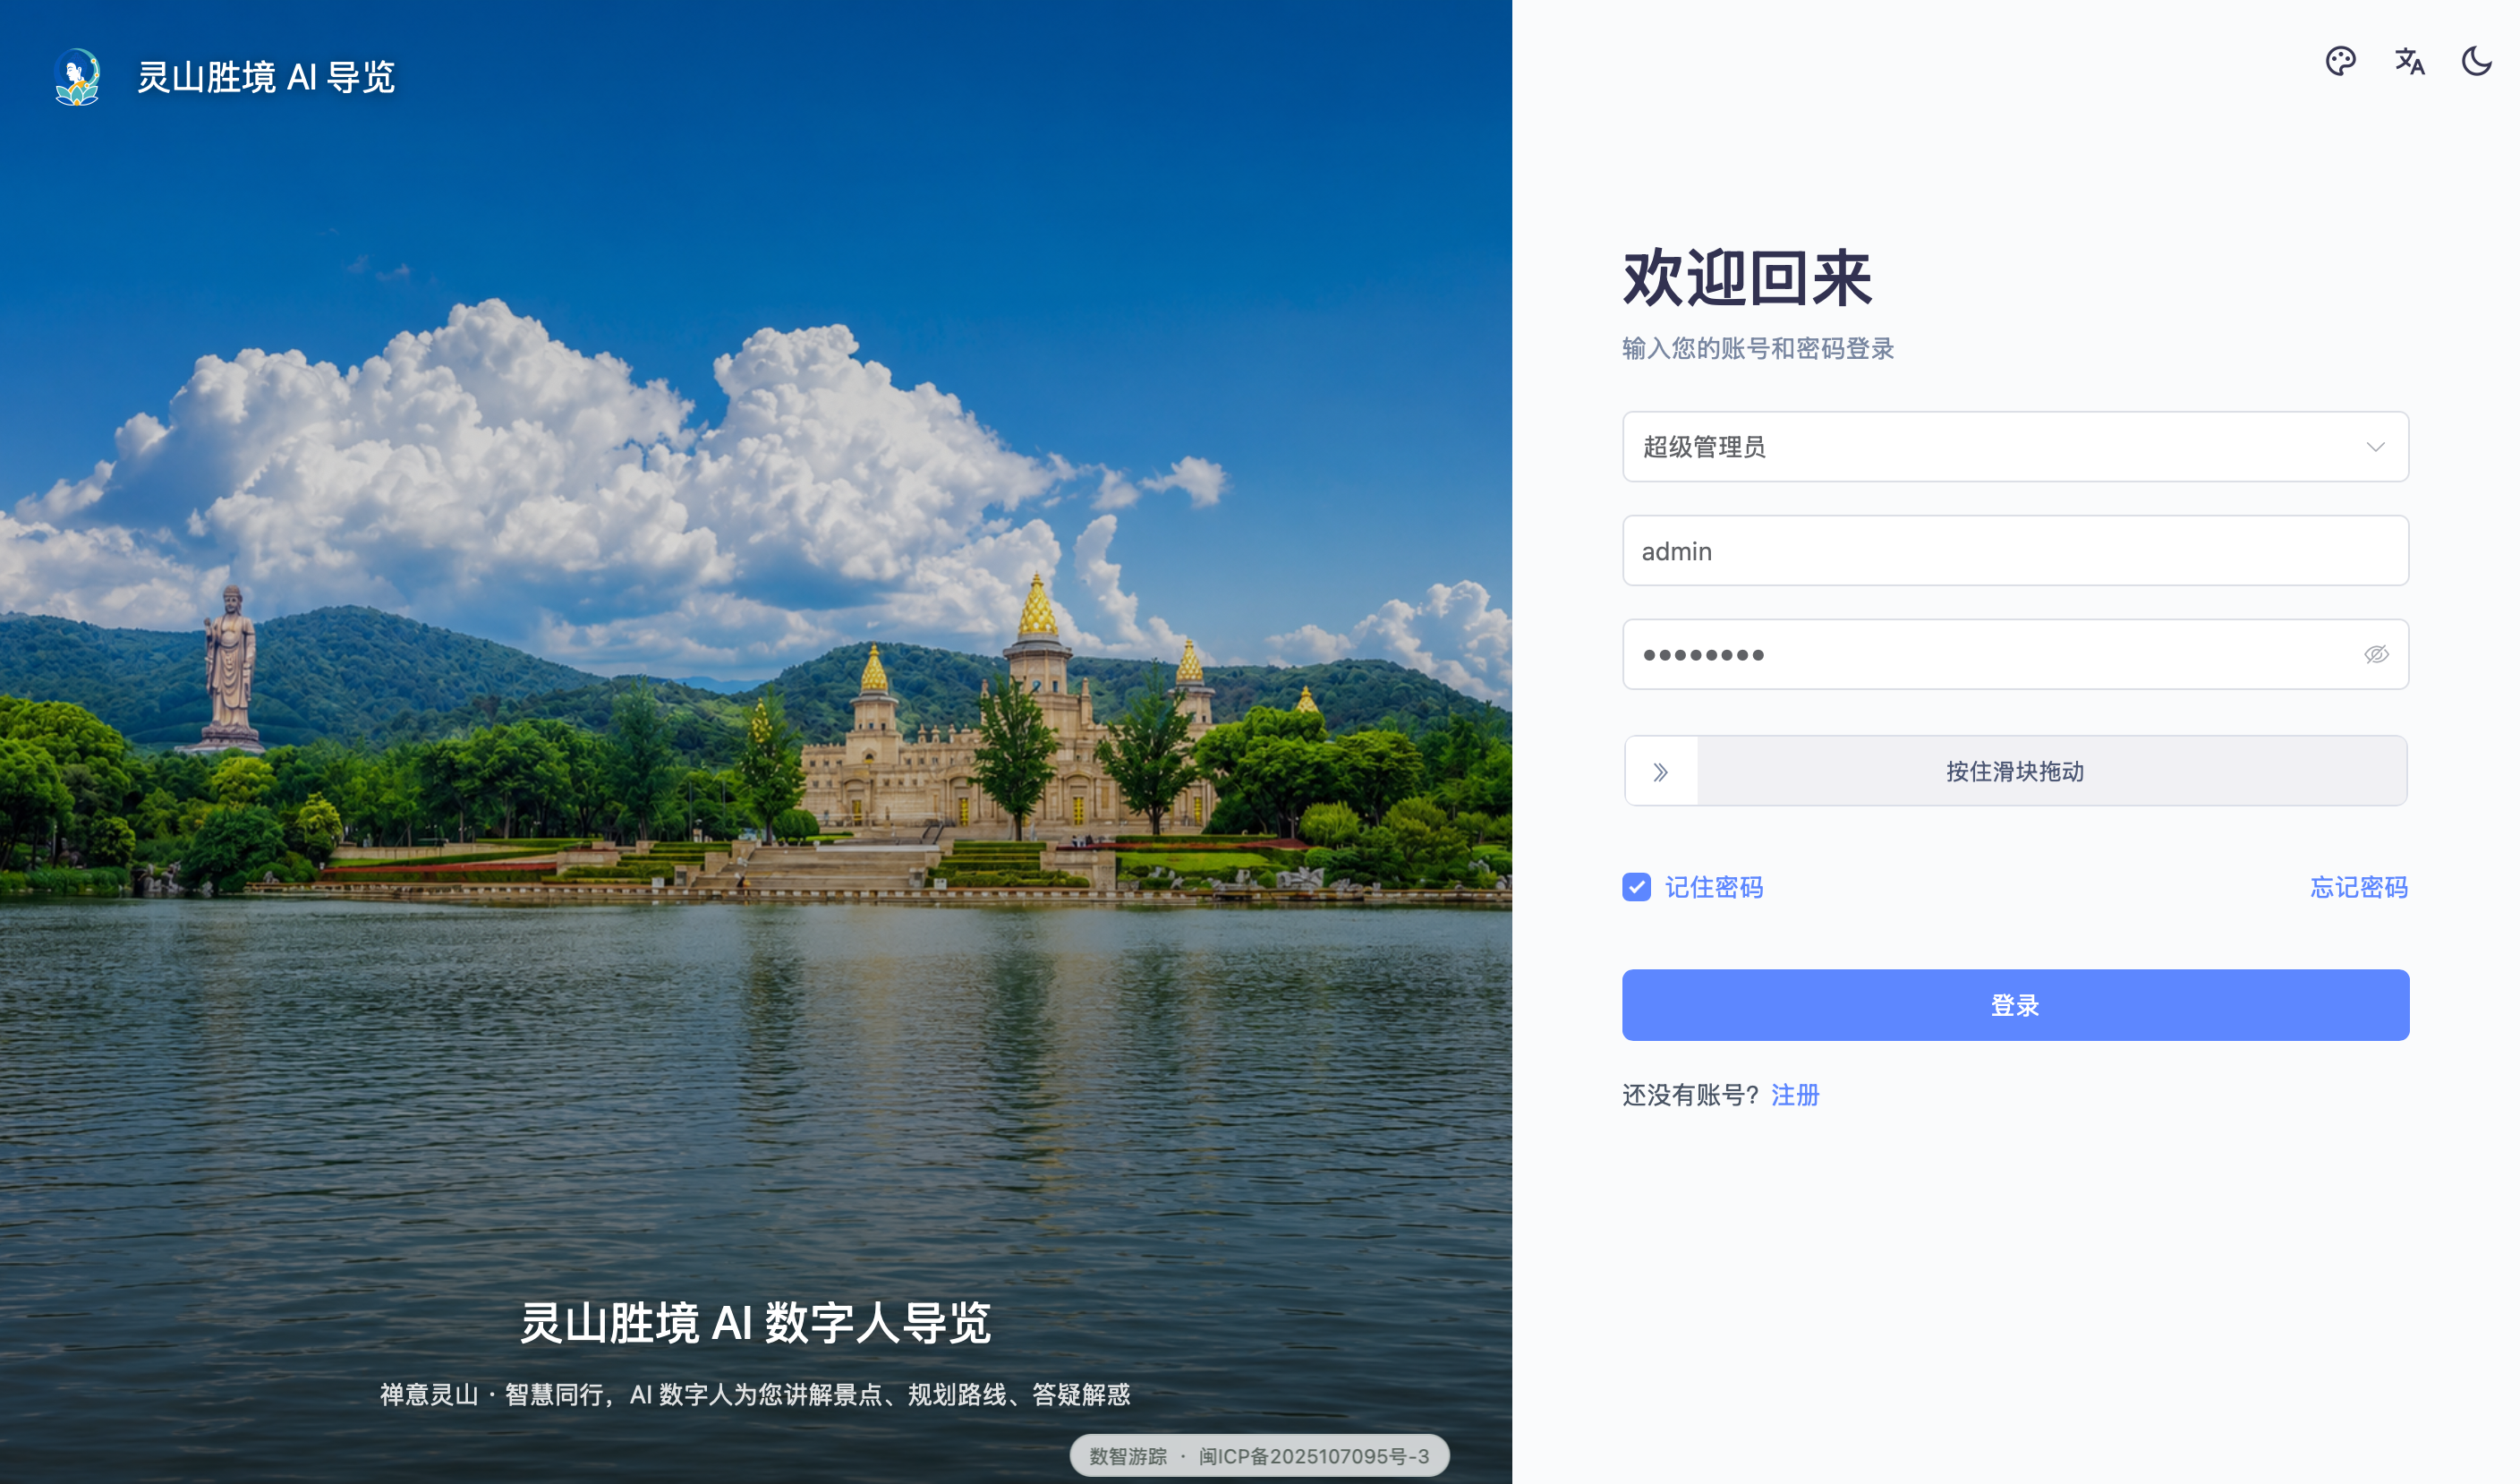
\includegraphics[width=0.95\textwidth]{assets/figures/login.png}%
  }{%
    \begin{tikzpicture}[x=1cm,y=1cm]
      \draw[rounded corners=5pt,very thick,guideTeal,fill=white] (0,0) rectangle (14.2,6.6);
      \fill[guideTeal] (0,0) rectangle (7.35,6.6);
      \node[text=white,font=\Large\bfseries] at (3.68,5.35) {数智游踪};
      \node[text=white,align=center,font=\small] at (3.68,4.60) {禅意灵山 · 智慧同行\\AI数字人景区导览与运营平台};
      \draw[white!65,rounded corners=3pt] (1.25,1.30) rectangle (6.10,3.75);
      \node[text=white,align=left,anchor=west] at (1.65,3.15) {\textbf{游客服务}\quad 问答 · 讲解 · 路线};
      \node[text=white,align=left,anchor=west] at (1.65,2.50) {\textbf{管理闭环}\quad 知识 · 数字人 · 运营};
      \node[text=white,align=left,anchor=west] at (1.65,1.85) {\textbf{可信保障}\quad 引用 · 质量 · 降级};
      \draw[rounded corners=5pt,thick,guideGray,fill=white] (8.15,0.65) rectangle (13.45,5.95);
      \node[font=\Large\bfseries,text=guideTeal] at (10.80,5.20) {管理端登录};
      \node[text=guideGray,font=\small] at (10.80,4.75) {账号验证后进入运营工作台};
      \node[anchor=west,font=\small] at (8.75,4.05) {用户名};
      \draw[rounded corners=2pt,guideGray] (8.75,3.40) rectangle (12.85,3.85);
      \node[anchor=west,text=guideGray,font=\small] at (8.95,3.62) {请输入管理员账号};
      \node[anchor=west,font=\small] at (8.75,2.95) {密码};
      \draw[rounded corners=2pt,guideGray] (8.75,2.30) rectangle (12.85,2.75);
      \node[anchor=west,text=guideGray,font=\small] at (8.95,2.52) {请输入登录密码};
      \draw[rounded corners=2pt,guideGold,fill=guideGoldLight] (8.75,1.55) rectangle (12.85,2.00);
      \node[text=guideGray,font=\small] at (10.80,1.77) {拖动滑块完成验证};
      \draw[rounded corners=2pt,guideTeal,fill=guideTeal] (8.75,0.90) rectangle (12.85,1.35);
      \node[text=white,font=\bfseries] at (10.80,1.12) {登录};
    \end{tikzpicture}%
  }
  \caption{管理端身份认证登录页面图}\label{fig:login-ui}
\end{figure}

\section{全局多语言交互}

页面右上角提供\textbf{统一语言入口}，语言选择作用于游客导览、知识库、数字人配置、运营大屏、会话反馈和系统管理等\textbf{全部路由}，而不是只替换顶部导航。切换动作同时更新\textbf{Vue i18n 活动语言与 Pinia 用户状态以}及 HTML 的\filepath{lang}属性，并通过版本化本地存储在下次访问时恢复。业务文案采用\textbf{五元组目录}维护，新增功能必须同时提供五种译文，降低遗漏单个页面或弹窗的风险。

\begin{table}[H]
  \centering
  \small
  \renewcommand{\arraystretch}{1.35}
  \caption{全局国际化语言与消息策略表}\label{tab:i18n-languages}
  \begin{tabularx}{\textwidth}{p{0.20\textwidth}p{0.13\textwidth}p{0.25\textwidth}X}
    \toprule
    界面语言 & 代码 & 基础消息来源 & 合并与回退策略 \\
    \midrule
    简体中文 & \texttt{zh} & \filepath{langs/zh.json} & 中文框架消息与完整业务消息目录 \\
    English & \texttt{en} & \filepath{langs/en.json} & 英文框架消息与完整业务消息目录，\newline 同时作为全局回退语言 \\
    韩文（Korean） & \texttt{ko} & 英文基础消息 & 合并韩文框架覆盖与韩文业务消息 \\
    繁體中文 & \texttt{zh-TW} & 简体中文基础消息 & 合并繁体框架覆盖与繁体业务消息 \\
    日本語 & \texttt{ja} & 英文基础消息 & 合并日文框架覆盖与日文业务消息 \\
    \bottomrule
  \end{tabularx}
\end{table}

\newpage
\section{游客端交互设计}

游客进入页面后由数字人播报欢迎语；可直接文字提问，也可启动语音输入。\textbf{Web端}按浏览器能力使用Web Speech API，\textbf{Android、iOS与HarmonyOS游客端}则由\filepath{uni.getRecorderManager}录音，经\filepath{uni.uploadFile}上传至\filepath{/api/voice/ask-upload}，从而复用服务端ASR--RAG--TTS链路；微信小程序在相同上传接口与权限约束下工作。问答结果同时呈现\textbf{答案、质量标签、来源和时延}，数字人按情绪标签播报。景点卡片触发约一分钟讲解，路线偏好面板采集时长、兴趣、亲子和拍照需求，结果节点可继续点击讲解。会话末尾支持\textbf{赞踩、1--5分和文字反馈}。

\begin{figure}[H]
  \centering
  \IfFileExists{assets/figures/visitor-guide.png}{%
    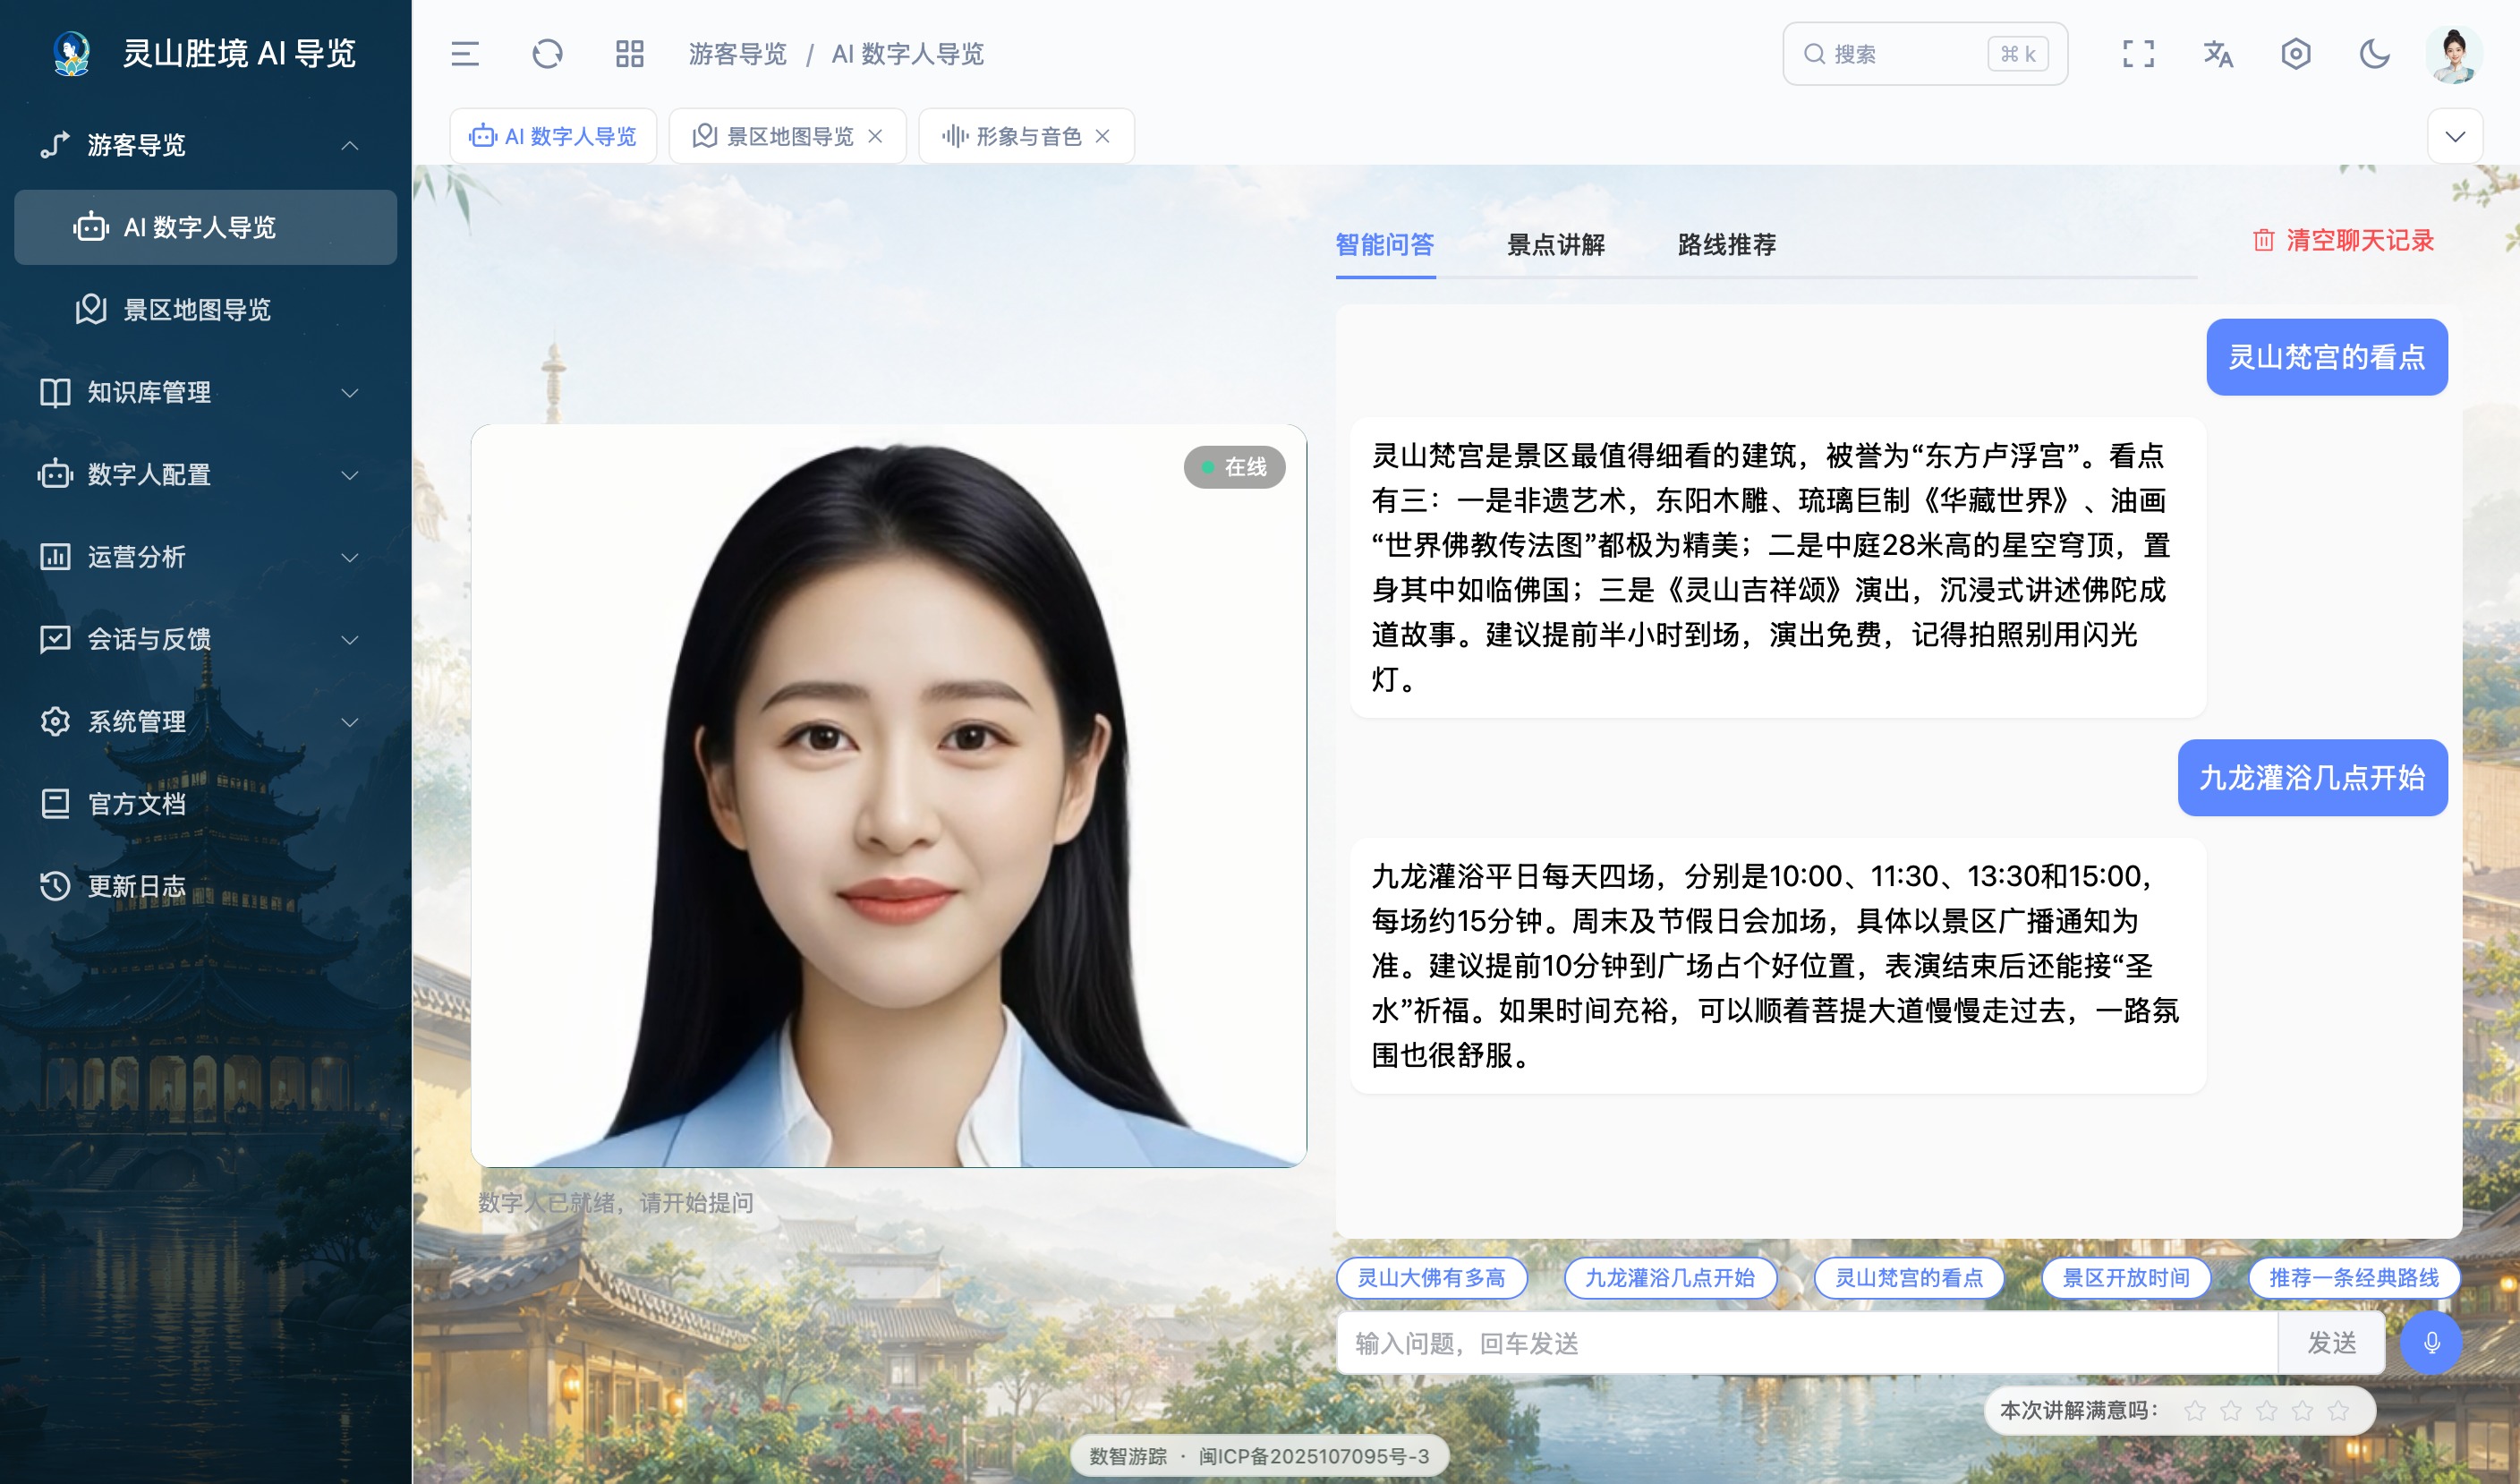
\includegraphics[width=0.95\textwidth]{assets/figures/visitor-guide.png}%
  }{%
    \begin{tikzpicture}[x=1cm,y=1cm]
      \draw[rounded corners=5pt,very thick,guideTeal,fill=guideTealLight] (0,0) rectangle (14.2,7.0);
      \fill[guideTeal] (0,6.35) rectangle (14.2,7.0);
      \node[anchor=west,text=white,font=\bfseries] at (0.35,6.68) {数智游踪 · 游客导览页截图占位};
      \draw[rounded corners=3pt,thick,guideTeal,fill=white] (0.45,0.55) rectangle (4.75,6.0);
      \node[align=center,font=\bfseries] at (2.60,5.55) {讯飞交互式数字人画面};
      \draw[dashed,guideGray] (1.10,1.50) rectangle (4.10,5.10);
      \node[align=center,text=guideGray] at (2.60,3.30) {实时视频流\\口型 / 表情 / 动作};
      \draw[rounded corners=3pt,thick,guideTeal,fill=white] (5.05,2.05) rectangle (9.45,6.0);
      \node[font=\bfseries] at (7.25,5.55) {问答与引用区};
      \draw[guideGray] (5.45,4.55) rectangle (9.05,5.20);
      \draw[guideGray] (5.45,3.55) rectangle (8.65,4.25);
      \draw[guideGray] (5.45,2.55) rectangle (9.05,3.20);
      \draw[rounded corners=3pt,thick,guideGold,fill=guideGoldLight] (9.75,2.05) rectangle (13.75,6.0);
      \node[font=\bfseries] at (11.75,5.55) {景点与路线区};
      \draw[guideGold] (10.15,4.55) rectangle (11.65,5.15);
      \draw[guideGold] (11.85,4.55) rectangle (13.35,5.15);
      \draw[guideGold] (10.15,3.55) rectangle (13.35,4.15);
      \draw[guideGold] (10.15,2.55) rectangle (13.35,3.15);
      \draw[rounded corners=3pt,thick,guideGray,fill=white] (5.05,0.55) rectangle (13.75,1.70);
      \node[text=guideGray] at (9.40,1.12) {文字/语音输入 · 快捷问题 · 满意度反馈};
    \end{tikzpicture}%
  }
  \caption{游客端AI数字人导览页面图}\label{fig:visitor-ui}
\end{figure}

\section{多端游客流程与界面适配}

游客端不是把桌面网页等比例缩小，而是以\textbf{同一业务服务、两套交互密度和按平台分支的系统能力}组织。Web与Electron桌面端保留数字人、引用、路线和地图的并列工作区，适合讲解大屏、游客中心与评审演示；uni-app x游客端使用“首页—地图—AI导游—行程—我的”五个底部入口，景点详情、账号、收藏和反馈按页面或微信分包加载。二者共享Node API、景点标识、会话结构和路线字段，但录音、定位、地图容器、WebView和文件上传分别调用浏览器或uni原生能力。

\begin{table}[H]
  \centering
  \small
  \caption{游客业务在不同终端的交互适配表}\label{tab:visitor-platform-adaptation}
  \begin{tabularx}{\textwidth}{p{0.15\textwidth}p{0.24\textwidth}p{0.25\textwidth}X}
    \toprule
    能力 & Web/桌面端 & Android/iOS/HarmonyOS & 微信小程序 \\
    \midrule
    语音输入 & Web Speech或页面录音能力，统一调用语音接口 & RecorderManager录音、uploadFile上传，服务端讯飞ASR & 同一录音上传链路，遵循小程序录音授权与包体约束 \\
    数字人 & 讯飞Web SDK在线形象，配置可切换Live2D & 受控HTTPS WebView承载讯飞形象，失败时回到本地表现与TTS & 个人主体与业务域名限制下不加载受限WebView，使用本地播报动画与讯飞云音色 \\
    地图定位 & 腾讯地图/Leaflet双路径，浏览器Geolocation & 原生\texttt{<map>}、本地手绘图与\texttt{uni.getLocation} & 原生\texttt{<map>}与GCJ-02定位，POI/算路由服务端Key能力补充 \\
    页面组织 & 多栏工作区，适合大屏和管理联动 & 五Tab移动信息架构，安全区和触控尺寸适配 & 主包五Tab，详情、账号、收藏与反馈拆为分包 \\
    \bottomrule
  \end{tabularx}
\end{table}

图\ref{fig:web-real-screens}和图\ref{fig:harmony-real-screens}均来自\textbf{当前可运行系统}，而非概念效果图。Web端展示数字人问答与景区手绘地图上的真实点位；HarmonyOS截图来自\textbf{HAP在Pura 90模拟器的安装运行结果}，覆盖首页、个人服务与AI导游主链路。Android APK与微信小程序的真实运行截图统一放在第\ref{sec:multiplatform-delivery}节，便于评审连续核对\textbf{多端交付结果}。

\begin{figure}[H]
  \centering
  \begin{minipage}[t]{0.65\textwidth}
    \centering
    
\includegraphics[width=\linewidth]{web-digital-human.png}
    \small Web在线数字人与问答界面
  \end{minipage}
  \par\medskip
  \begin{minipage}[t]{0.65\textwidth}
    \centering
    
\includegraphics[width=\linewidth]{web-scenic-map.png}
    \small Web景区点位与手绘地图界面
  \end{minipage}
  \caption{Web端真实运行界面组图}\label{fig:web-real-screens}
\end{figure}

\begin{figure}[H]
  \centering
  \begin{minipage}[t]{0.30\textwidth}
    \centering
    
\includegraphics[width=\linewidth]{visitor-harmony-home.png}
    \small 首页与景点入口
  \end{minipage}\hfill
  \begin{minipage}[t]{0.30\textwidth}
    \centering
    
\includegraphics[width=\linewidth]{visitor-harmony-infor.png}
    \small “我的”与个人服务页面
  \end{minipage}\hfill
  \begin{minipage}[t]{0.30\textwidth}
    \centering
    
\includegraphics[width=\linewidth]{visitor-harmony-ai.png}
    \small AI导游与数字人入口
  \end{minipage}
  \caption{HarmonyOS HAP真实运行界面组图}\label{fig:harmony-real-screens}
\end{figure}

\section{多模态交互流程}

图\ref{fig:multimodal-flow}将\textbf{核心节点固定在同一水平线上}。快捷问题、云端数字人和会话记录作为扩展节点位于两侧，曲线从节点边缘出发，不穿越核心内容。

\begin{figure}[H]
  \centering
  \resizebox{0.98\textwidth}{!}{%
  \begin{tikzpicture}[x=1cm,y=1cm]
    \node[core] (m1) at (0,0) {游客输入\\语音或文本};
    \node[core] (m2) at (3.05,0) {输入标准化\\ASR/文本};
    \node[core] (m3) at (6.10,0) {可信问答\\FAQ/RAG/LLM};
    \node[coregold] (m4) at (9.15,0) {数字人表达\\TTS/口型/表情};
    \node[coregold] (m5) at (12.20,0) {反馈沉淀\\评分与会话};
    \draw[flow] (m1.east) -- (m2.west);
    \draw[flow] (m2.east) -- (m3.west);
    \draw[flowgold] (m3.east) -- (m4.west);
    \draw[flowgold] (m4.east) -- (m5.west);
    \node[side] (quick) at (0,2.0) {快捷问题\\景点卡片};
    \node[side] (sdk) at (9.15,-2.0) {讯飞WebRTC\\形象与音色};
    \node[side] (admin) at (12.20,2.0) {后台分析\\质量与趋势};
    \draw[curved] (quick.south) to[out=270,in=90] (m1.north);
    \draw[curved] (m3.south) to[out=270,in=180] (sdk.west);
    \draw[curved] (sdk.north) to[out=90,in=270] (m4.south);
    \draw[curved] (m5.north) to[out=90,in=270] (admin.south);
  \end{tikzpicture}}
  \caption{语音文本与数字人协同交互流程图}\label{fig:multimodal-flow}
\end{figure}

\newpage
\section{管理端交互设计}

管理端按业务闭环设置\textbf{六组菜单}：知识库管理、数字人配置、运营分析、会话与反馈、服务质量、系统用户。\\运营人员可在\textbf{不修改代码}的情况下维护FAQ与景点资料，并在数字人新增/编辑弹窗中展开\textbf{“选择形象”和“选择音色”}目录。选择形象会同步填入讯飞\filepath{avatarId}或Live2D \filepath{modelId}及角色名称，选择音色会写入\textbf{VCN参数}；下方表单继续支持欢迎语、语速、情绪风格、服务状态和启用开关等精细配置。

\subsection{形象模型与音色目录}

系统内置\textbf{四组讯飞云端形象和四组Live2D本地模型}，名称同时标明\textbf{性别与赛题景区元素}，便于运营人员快速判断使用场景。启用任一配置后，游客端通过\textbf{同一接口}读取并选择对应渲染引擎。

\begin{table}[H]
  \centering
  \small
  \caption{数字人快捷形象目录}\label{tab:avatar-catalog}
  \begin{tabularx}{\textwidth}{p{0.17\textwidth}p{0.27\textwidth}p{0.10\textwidth}X}
    \toprule
    引擎 & 形象名称 & 性别 & 运行标识 \\
    \midrule
    讯飞云端 & 景行·灵山迎宾使 & 男 & \texttt{cnr5dg8n2000000003} \\
    讯飞云端 & 灵悦·莲心礼宾使 & 女 & \texttt{cnrfb86h2000000004} \\
    讯飞云端 & 云觉·大佛文化使 & 女 & \texttt{cnrmkf0e2000000006} \\
    讯飞云端 & 梵音·梵宫导览使 & 女 & \texttt{cnrn9jgi2000000005} \\
    Live2D本地 & 春和·九龙灵使 & 女 & \texttt{Haru} \\
    Live2D本地 & 晴音·莲华旅伴 & 女 & \texttt{Hiyori} \\
    Live2D本地 & 知远·坛城研学使 & 男 & \texttt{Kei} \\
    Live2D本地 & 清响·禅旅伙伴 & 男 & \texttt{Hibiki} \\
    \bottomrule
  \end{tabularx}
\end{table}

音色目录既包含发言人管理资料中的\textbf{英语、台湾腔和东北话音色}，也保留项目导览链路使用的普通话男女声。界面同时展示\textbf{可读名称、语种和原始VCN}，确保配置参数与讯飞账号权限能够逐项核对。

\begin{table}[H]
  \centering
  \small
  \caption{数字人快捷音色目录}\label{tab:voice-catalog}
  \begin{tabularx}{\textwidth}{p{0.23\textwidth}p{0.22\textwidth}X}
    \toprule
    音色 & 语种/口音 & VCN参数 \\
    \midrule
    Grant & 美式英语 & \filepath{x5_EnUs_Grant_flow} \\
    台湾腔温柔男声 & 台湾普通话 & \filepath{x6_taiqiangnuannan_pro} \\
    Lila & 美式英语 & \filepath{x5_EnUs_Lila_flow} \\
    子阳 & 东北话 & \filepath{x4_ziyang_oral} \\
    聆小玥 & 普通话 & \filepath{x5_lingxiaoyue_flow} \\
    鹏飞 & 普通话 & \filepath{x4_pengfei} \\
    导览女声 & 普通话 & \filepath{x6_jingqudaolannvsheng_mini} \\
    导览男声 & 普通话 & \filepath{x6_zhantingnanjiedai_pro} \\
    \bottomrule
  \end{tabularx}
\end{table}

\begin{figure}[H]
  \centering
  \IfFileExists{web-operations-dashboard.png}{%
    
\includegraphics[width=0.86\textwidth]{web-operations-dashboard.png}%
  }{\IfFileExists{assets/figures/admin-dashboard.png}{%
    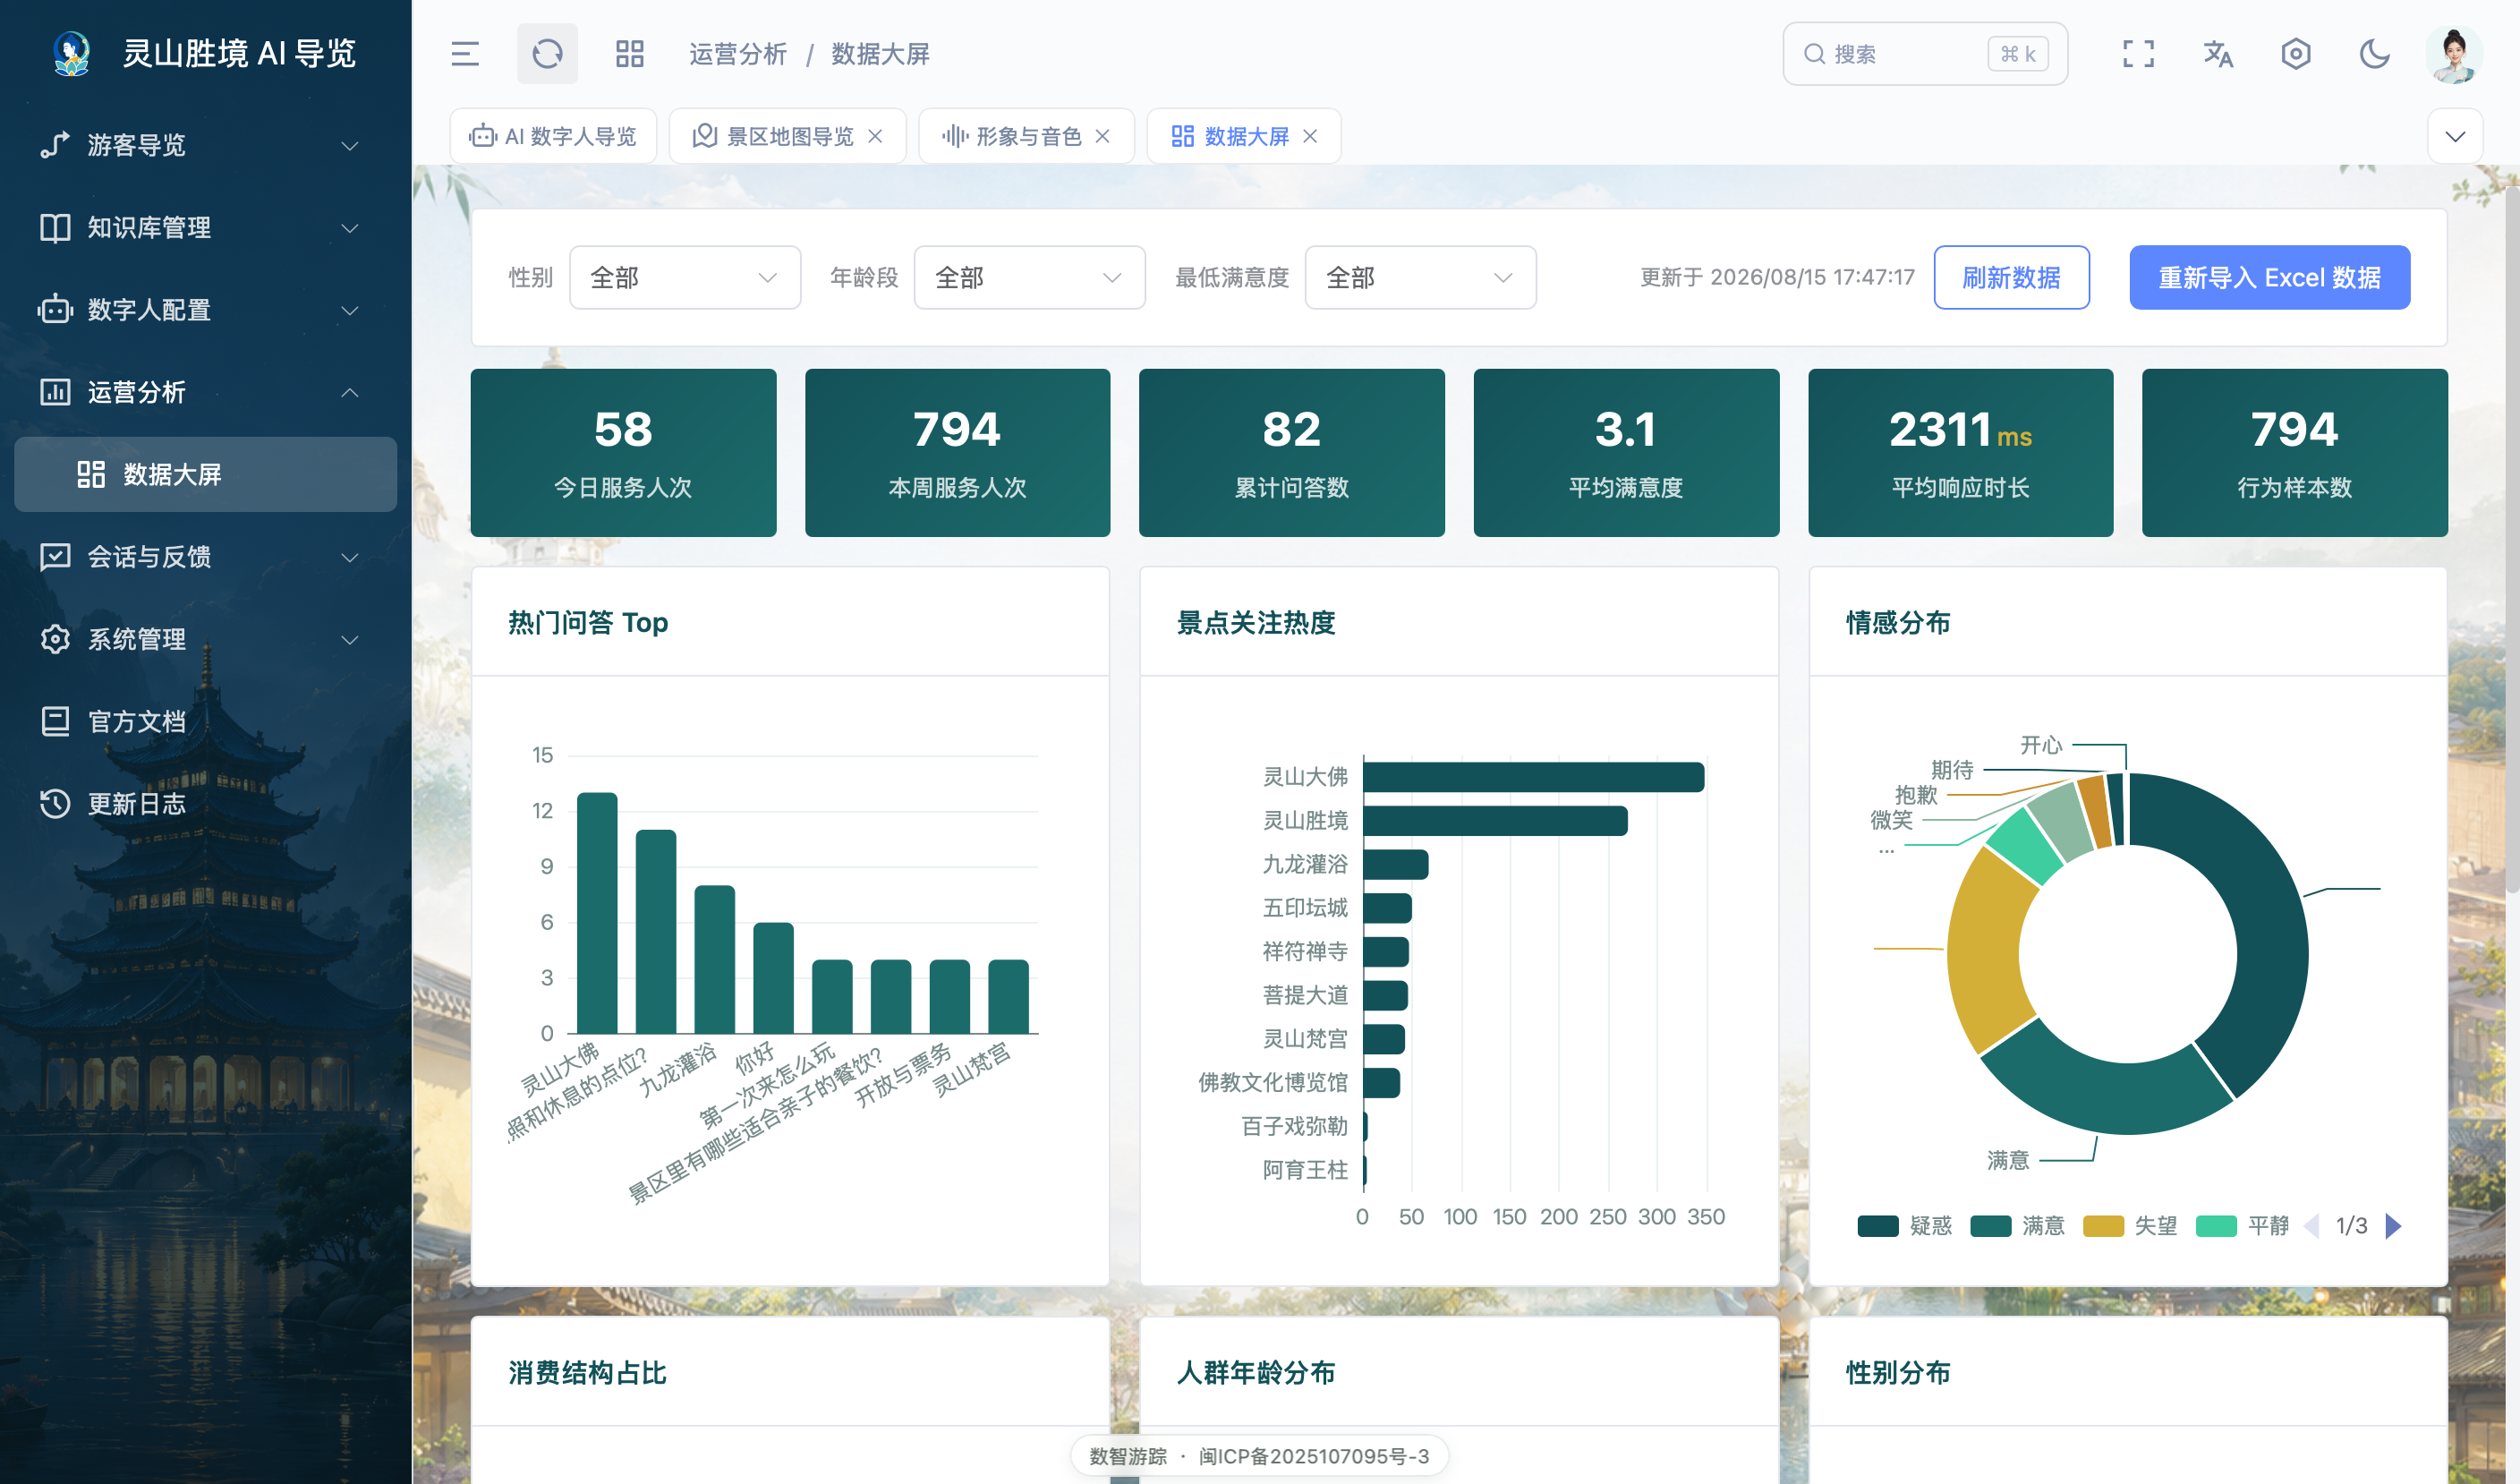
\includegraphics[width=0.86\textwidth]{assets/figures/admin-dashboard.png}%
  }{%
    \begin{tikzpicture}[x=1cm,y=1cm]
      \draw[rounded corners=5pt,very thick,guideGold,fill=guideGoldLight] (0,0) rectangle (14.2,6.9);
      \fill[guideTeal] (0,0) rectangle (2.2,6.9);
      \node[text=white,font=\bfseries,align=center] at (1.1,6.35) {数智游踪\\管理后台};
      \foreach \y/\t in {5.45/知识库管理,4.65/数字人配置,3.85/运营分析,3.05/会话与反馈,2.25/服务质量,1.45/系统管理}{
        \node[text=white,anchor=west,font=\small] at (0.38,\y) {\t};
      }
      \draw[rounded corners=3pt,fill=white,draw=guideGold] (2.55,5.25) rectangle (5.15,6.35);
      \draw[rounded corners=3pt,fill=white,draw=guideGold] (5.45,5.25) rectangle (8.05,6.35);
      \draw[rounded corners=3pt,fill=white,draw=guideGold] (8.35,5.25) rectangle (10.95,6.35);
      \draw[rounded corners=3pt,fill=white,draw=guideGold] (11.25,5.25) rectangle (13.85,6.35);
      \node at (3.85,5.80) {服务人次}; \node at (6.75,5.80) {满意度};
      \node at (9.65,5.80) {平均时延}; \node at (12.55,5.80) {问答总量};
      \draw[rounded corners=3pt,fill=white,draw=guideGold] (2.55,2.95) rectangle (8.05,4.90);
      \draw[rounded corners=3pt,fill=white,draw=guideGold] (8.35,2.95) rectangle (13.85,4.90);
      \draw[guideTeal,very thick] (3.05,3.35) -- (4.10,4.05) -- (5.15,3.75) -- (6.20,4.45) -- (7.55,4.15);
      \node[text=guideGray] at (5.30,3.10) {趋势与景点热度};
      \draw[fill=guideTealLight,draw=guideTeal] (8.90,3.35) rectangle (9.55,4.30);
      \draw[fill=guideGoldLight,draw=guideGold] (9.90,3.35) rectangle (10.55,4.60);
      \draw[fill=guideTealLight,draw=guideTeal] (10.90,3.35) rectangle (11.55,4.05);
      \draw[fill=guideGoldLight,draw=guideGold] (11.90,3.35) rectangle (12.55,4.40);
      \draw[rounded corners=3pt,fill=white,draw=guideGold] (2.55,0.55) rectangle (13.85,2.55);
      \node[text=guideGray] at (8.20,1.55) {消费结构 · 游客画像 · 热门问题 · 运营建议};
    \end{tikzpicture}%
  }}
  \caption{管理端运营分析大屏页面图}\label{fig:admin-ui}
\end{figure}

图\ref{fig:admin-ui}把服务人次、满意度、平均时延、问答总量、景点热度、游客画像和运营建议放在同一观察面板中。它与上文的知识库、数字人配置和会话反馈入口形成\textbf{“配置—服务—观察—修正”}闭环，评审时可以沿同一页面理解管理端如何把游客数据转化为内容维护动作。
